\chapter{Background Research}\label{ch:backgroundresearch}
Hello\todo{add intro to BGres}

\section{Visual Depth Perception Within Humans}
Hello\todo{add section here}

\section{Cognition, Experiential Learning, and Learning Styles}
Hello\todo{add section here}

\section{Augmented Reality}
As suggested by Madden in the book Professional Augmented Reality Browsers for Smartphones, AR is to be thought of as the opposite of Virtual Reality (VR). As Madden explains it: “Virtual reality immerses the user in a computer-generated world whereas AR combines the real world with computer graphics.” \cite{Madden2011}. Moreover, Madden points out that where it requires the user to acquire special equipment to experience VR, AR requires only a device able to capture the environment (e.g. a smartphone or tablet) as well as methods to experience the computer world typically in the form of an overlaying computer graphic in the camera window \cite{Madden2011}. Based on this, Madden defines AR as a technology which combines the real world with computer graphics, tracking and/or providing interaction with objects in real-time. Furthermore, AR provides recognition of images or objects, as well as delivering real-time context or data. By utilising this definition Madden allows technologies to be included that are not considered AR in the strictest interpretations e.g. AR browsers \cite{Madden2011}.

In relation to the above definition of AR, Madden makes a distinction between two tracking systems, namely tracking by markers and markerless tracking. The method of tracking by markers makes use of patterned images, which activate a certain action when recognised. Examples of markers are the fiduciary marker, Quick response codes (QR), and Microsoft Tags. Markerless tracking on the other hand works by tracking objects in the real world not using markers made for the purpose. An example of markerless tracking is facial recognition \cite{Madden2011}.

Approaches to mobile AR are mainly split into two paths, namely AR using location and orientation data to compute what is viewed, and AR using actual image content captured by a camera to compute what is viewed referred to as \textit{computer vision}.

As introduced by Madsen and Lal, Aalborg University, in the book Augmented Reality, chapter 2 \cite{Lal2010}, AR can be associated with three major challenges:

\begin{enumerate}
\item Camera tracking 
\item Handling occlusions
\item Illumination consistency
\end{enumerate}

The obstacle with camera tracking involves \textit{“matching position and orientation of the camera to the coordinate system of the scene”} \cite{Lal2010}, which deals with making sure the angle of the scene captured by the camera matches that of the virtual scene. Handling occlusions means \textit{“having sufficient 3D information of the real scene to handle occlusion between real and virtual geometry”} \cite{Lal2010}, so that real-world objects such as people walking by may occlude the virtual objects. Lastly, illumination consistency deals with the problems of \textit{“having sufficient knowledge of the real scene illumination to be able to render virtual objects with scene consistent illumination, including shadows”} \cite{Lal2010}. The latter of these three is especially important for creating visually credible AR in outdoor environments because of this scenario’s dynamically changing illumination.

\section{State of the Art}
Augmented reality can be used to various ends. The popular game Pokémon Go, which was released in the summer of 2016, includes an optional AR feature \cite{Pokemon}. However, AR has also been utilised for tourism. Feiner et al. (1997) developed a system which allowed users to access access information about a campus using an overlay interface \cite{Feiner1997}. Because of the age of this prototype, however, a bulky setup was required, including a backpack-worn computer and a head-mounted display. A prototype built by Fritz et al. (2005) uses a camera, binoculars and internal sensors to augment a video stream with graphical objects, such as information of a site, or visualisations of what a site looked like in the past \cite{Fritz2005}. A sketch of this prototype is seen in Figure \ref{fig:binoculars}.

\begin{figure}[h!]
    \centering
    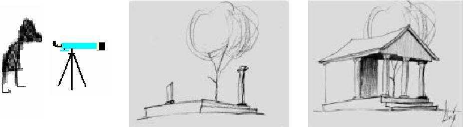
\includegraphics[scale=1]{figures/binoc.png}
    \caption{Sketch of Fritz et al.'s prototype (left), the unaugmented image (middle), and the augmented image (right) \cite{Fritz2005}}\label{fig:binoculars}
\end{figure}

While a majority of AR solutions for tourists are scientific prototypes, a few commercial products are available for mobile smartphones. Using apps such as Wikitude, users can experience several different types of AR experiences, as developers are able to upload their AR project to the platform. This allows various third-party stakeholders to utilise the app. A screenshot of Tripadvisor's use of the Wikitude platform can be seen in Figure \ref{fig:wikitude}. The app uses different input methods to load the AR experiences, such as GPS location, images, and QR-codes \cite{Wikitude}. It primarily functions as a platform for AR advertisements or similar commercial products.

\begin{figure}[h!]
    \centering
    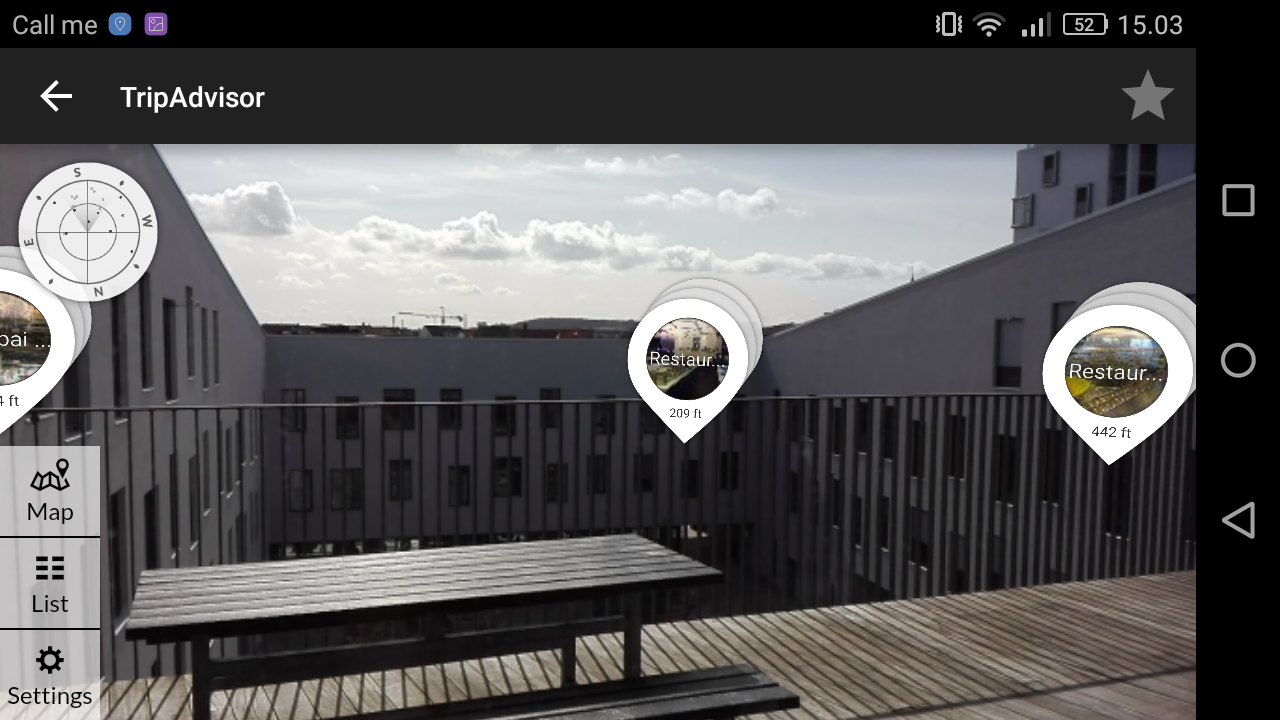
\includegraphics[width=0.7\textwidth]{figures/wikitude.png}
    \caption{Screenshot of the Wikitude app, as utilised by Tripadvisor}\label{fig:wikitude}
\end{figure}

The Yelp app, dedicated to reading and writing reviews of local restaurants, has an optional feature called \textit{monocle}, which allows users to see the average rating of nearby restaurants based on location \cite{Yelp}. A downside to this feature is that depending on the density of nearby restaurants, the screen may get quite cluttered, as can be seen in Figure \ref{fig:yelp}.

\begin{figure}[h!]
    \centering
    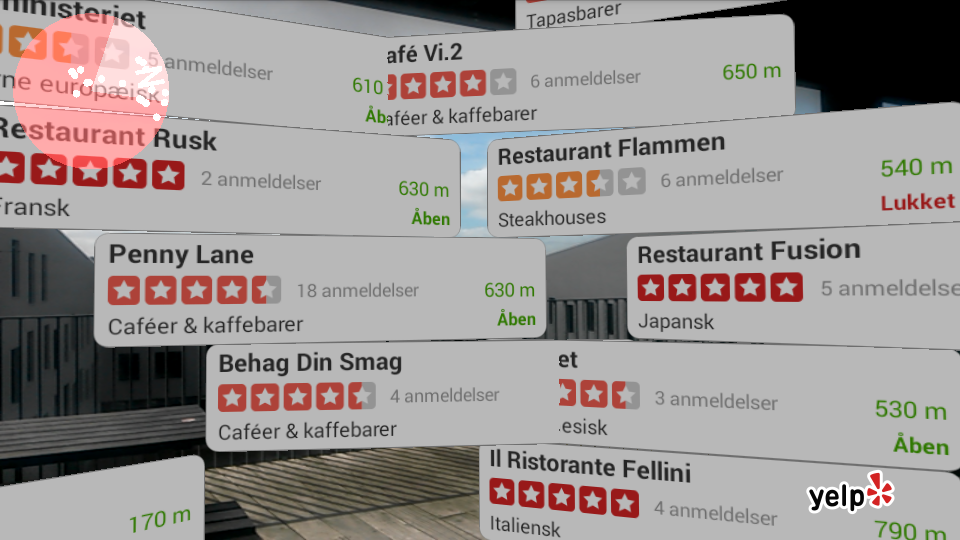
\includegraphics[width=0.7\textwidth]{figures/yelp.png}
    \caption{Screenshot of the Yelp monocle feature}\label{fig:yelp}
\end{figure}

%I am just commenting this out in case we need it
%Here is equation~\eqref{eq:esun}:

%\begin{equation}
%\label{eq:esun}
%E_{sun} = (\vec{n} \cdot \vec{s}) \times \_E_{sun}
%\end{equation}